\documentclass[hide notes,intlimits,handout]{beamer}

\mode<presentation>
{
  \usetheme[footline]{UAFshade}
  \setbeamercovered{transparent}
}

% load packages
\usepackage[english]{babel}
\usepackage[latin1]{inputenc}
\usepackage[T1]{fontenc}
\usepackage{lmodern}
\usepackage{multimedia}
%\usepackage{hyperref}

% Some useful commands (from ELB)
\newcommand{\bD}{\mathbf{D}}
\newcommand{\bbf}{\mathbf{f}}
\newcommand{\bF}{\mathbf{F}}
\newcommand{\bg}{\mathbf{g}}
\newcommand{\bn}{\mathbf{n}}
\newcommand{\bq}{\mathbf{q}}
\newcommand{\bT}{\mathbf{T}}
\newcommand{\bu}{\mathbf{u}}
\newcommand{\bU}{\mathbf{U}}
\newcommand{\bv}{\mathbf{v}}

\newcommand{\ddx}[1]{\ensuremath{\frac{\partial #1}{\partial x}}}
\newcommand{\ddy}[1]{\ensuremath{\frac{\partial #1}{\partial y}}}
\newcommand{\ddz}[1]{\ensuremath{\frac{\partial #1}{\partial z}}}
\newcommand{\ddt}[1]{\ensuremath{\frac{\partial #1}{\partial t}}}

\newcommand{\DDt}[1]{\ensuremath{\frac{d #1}{d t}}}

\newcommand{\Div}{\nabla\cdot}
\newcommand{\eps}{\epsilon}
\newcommand{\grad}{\nabla}
\newcommand{\half}{\frac{1}{2}}
\newcommand{\trace}{\operatorname{tr}}

\newcommand{\rinv}{\frac{1}{r}}
\newcommand{\ar}{r^{-1}\alpha}
\newcommand{\stress}{\ensuremath{\text{\Large$\sigma$\normalsize}}}
\newcommand{\devstress}{\ensuremath{\text{\Large$\tau$\normalsize}}}

% Some useful commands (from MPL)
\newcommand{\s}[1]{\ensuremath{\,\text{#1}}}
\newcommand{\unit}[1]{\ensuremath{\,\text{#1}}}




% title page
\title[Glacier Thermodynamics] % (optional, use only with long paper titles)
{Thermodynamics of Glaciers}
\subtitle{McCarthy Summer School}


\author[Aschwanden] % (optional, use only with lots of authors)
{Andy Aschwanden}
% - Give the names in the same order as the appear in the paper.
% - Use the \inst{?} command only if the authors have different
%   affiliation.

\institute[ARSC] % (optional, but mostly needed)
{
  %
  Arctic Region Supercomputing Center\\
  University of Alaska Fairbanks, USA
}
% - Use the \inst command only if there are several affiliations.
% - Keep it simple, no one is interested in your street address.

\date{June 2012}

\titlegraphic{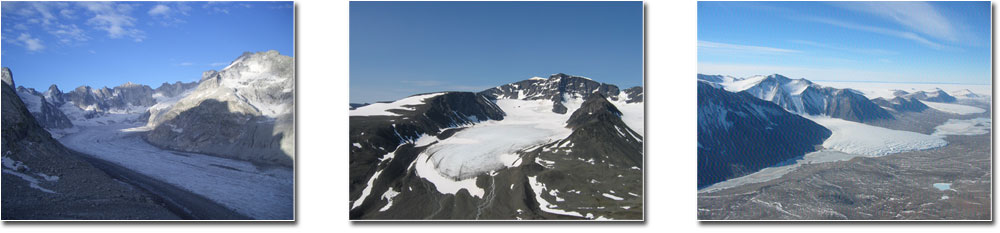
\includegraphics[width=10cm]{figures/glaciers3}}


\subject{Glaciers}

\begin{document}

\AtBeginSection[]
{
  \begin{frame}<handout:0>
    \frametitle{Outline}
    \tableofcontents[sectionstyle=show/shaded,subsectionstyle=hide]
  \end{frame}
}


% insert titlepage
\begin{frame}
  \titlepage
\end{frame}



\section{Introduction}
\label{sec:introduction}

\begin{frame}
  \frametitle{On Notation}
  \begin{itemize}
  \item (hopefully) consistent with Continuum Mechanics (Truffer)
  \item with lots of input from \emph{Luethi \& Funk: Physics of Glaciers I} lecture at ETH
  \item notation following Greve \& Blatter: Dynamics of Ice Sheets and Ice Sheets
  \end{itemize}
  \begin{figure}
    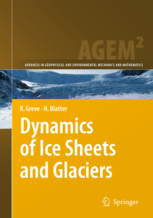
\includegraphics[scale=1.25]{figures/greveblatter_disg}
  \end{figure}
\end{frame}


\frame<handout:0>{
  \begin{figure}
    \includegraphics<1>[width=11cm]{figures/glacier_opaque}%
    \includegraphics<2>[width=11cm]{figures/glacier_temp}%
    \includegraphics<3>[width=11cm]{figures/glacier_poly}%
    \includegraphics<4>[width=11cm]{figures/glacier_cold}%    
  \end{figure}
  \begin{overlayarea}{4cm}{.5cm}
    \only<2>{\small Photo: A. Aschwanden}
    \only<3>{\small Photo: R. Hock}
    \only<4>{\small Photo: S. White}  
  \end{overlayarea}
}

\begin{frame}
  \frametitle{Types of Glaciers}
  \begin{columns}
    \column[C]{2.25cm}
    \begin{figure}
      \includegraphics<1>[width=2cm]{figures/taylor_valley_w}
    \end{figure}      
    \column[C]{9.5cm}
    \begin{block}
      {cold glacier} ice below pressure melting point, no liquid water
    \end{block}
  \end{columns}
  \begin{columns}
    \column[C]{2.25cm}
    \begin{figure}
      \includegraphics<1>[width=2cm]{figures/forno_w}%
    \end{figure}
    \column[C]{9.5cm}
    \begin{block}
      {temperate glacier} ice at pressure melting point, contains liquid water in the ice matrix
    \end{block}
  \end{columns}
  \begin{columns}
    \column[C]{2.25cm}
    \begin{figure}
      \includegraphics<1>[width=2cm]{figures/stor_w}
    \end{figure}     
    \column[C]{9.5cm}
    \begin{block}
      {polythermal glacier} cold and temperate parts
    \end{block}
  \end{columns}
  \note{
    \begin{itemize}
    \item these 3 glaciers serve as examples of 3 glacier types
    \end{itemize}
  }   
\end{frame}


\begin{frame}
  \frametitle{Why we care}
  The knowledge of the distribution of temperature in glaciers and ice sheets is of high practical interest
  \begin{itemize}[<+-| alert@+>]
  \item A temperature profile from a cold glacier contains information on past
    climate conditions.
  \item Ice deformation is strongly dependent on temperature (temperature
    dependence of the rate factor $A$ in Glen's flow law); 
  \item The routing of meltwater through a glacier is affected by ice
    temperature.  Cold ice is essentially impermeable, except for discrete
    cracks and channels.
  \item If the temperature at the ice-bed contact is at the pressure melting
    temperature the glacier can slide over the base.
  \item Wave velocities of radio and seismic signals are temperature
    dependent. This affects the interpretation of ice depth soundings.
  \end{itemize}
\end{frame}


\section{Energy balance}
\label{sec:energy-balance}

\begin{frame}
  \frametitle{Energy balance: depicted}
  \begin{figure}
    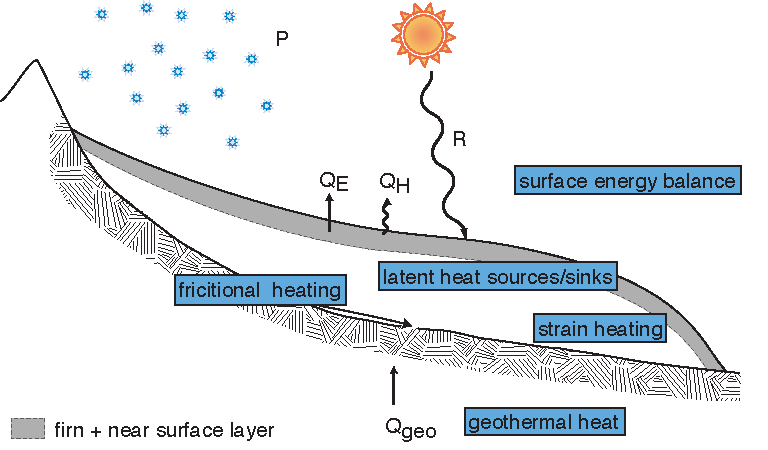
\includegraphics[width=10cm]{figures/glacier_thermodynamics}
  \end{figure}
\end{frame}


\begin{frame}
  \frametitle{Energy balance: equation}
  \begin{columns}
    \column[c]{7cm}
    \begin{equation*}
      \rho \left(\ddt{u} + \bv \cdot \grad u\right) = - \Div \bq + Q
    \end{equation*}
   \vspace{2em}
    \column[c]{6cm}
      \begin{tabular}{cl}
        $\rho$ \quad & ice density \\
        u \quad & internal energy \\
        $\bv$ \quad & velocity \\
        $\bq$ \quad & heat flux \\
        $Q$ \quad & dissipation power \\
             & (strain heating)
      \end{tabular}
    \end{columns}
    \begin{block}{Noteworthy}
      \begin{itemize}
      \item strictly speaking, internal energy is \alert{not} a conserved quantity
      \item only the sum of \alert{internal energy} and \alert{kinetic energy} is a conserved quantity
      \end{itemize}
    \end{block}
\end{frame}


\section{Cold Ice}
\label{sec:cold-ice}

\subsection{Equation}
\label{sec:cold-ice-equation}

\begin{frame}
  \frametitle{Temperature equation}
  \begin{columns}
    \column[c]{1.75cm} 
    \vspace{1cm}
    {\includegraphics<1>[width=1.5cm]{figures/glaciersv_c}}%
    \column[c]{10.25cm}
    \begin{block}{Temperature equation}
      \begin{itemize}
        \item ice is cold if a change in heat content leads to a change in temperature alone
        \item independent variable: temperature $T = c(T)^{-1} u$
        \end{itemize}
      \begin{equation*}
        \label{eq:cold_pde}
        \rho c(T)\left(\ddt{T} + {\bf v}\cdot\nabla T\right) =  - \nabla \cdot {\bf q} + Q
      \end{equation*}
   \end{block}
   \begin{block}{Fourier-type sensible heat flux}
      \begin{equation*}
        \label{eq:enthalpy-flux-cold}
        {\bf q}  = {\bf q}_{s} = -k(T)\nabla T
      \end{equation*}
    \end{block}
    \begin{tabular}{cl}
      $c(T)$ & heat capacity \\
      $k(T)$ & thermal conductivity \\
    \end{tabular}
  \end{columns}  
\end{frame}

\subsection{Thermal properties}
\label{sec:cold-ice-thermal-properties}

\begin{frame}
  \frametitle{Thermal properties}
  \begin{columns}
    \column[c]{1.75cm} 
    \vspace{1cm}
    {\includegraphics<1>[width=1.5cm]{figures/glaciersv_c}}%
    \column[c]{10.25cm}
    \begin{columns}
      \column[c]{5.5cm} 
      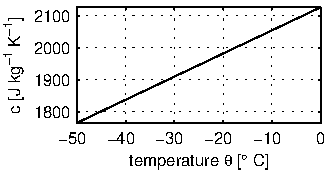
\includegraphics[5.cm]{figures/c}
      \column[c]{4cm}
      \alert{heat capacity} is a monotonically-increasing function of temperature
    \end{columns}  
    \begin{columns}
      \column[c]{5.5cm} 
      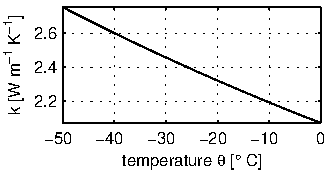
\includegraphics[5cm]{figures/k}
      \column[c]{4cm}
      \alert{thermal conductivity} is a monotonically-decreasing function of temperature
    \end{columns}  
  \end{columns}  
\end{frame}


\subsection{Flow law}
\label{sec:cold-ice-flow-law}

\begin{frame}
  \frametitle{Flow law}
  \begin{columns}
    \column[T]{1.75cm} 
    \vspace{1cm}
    {\includegraphics<1>[width=1.5cm]{figures/glaciersv_c}}%
    \vspace{2.5cm}
    \column[T]{10.25cm}
     Viscosity $\eta$ is a function of effective strain rate $d_{\text e}$  and temperature $T$
      \begin{equation*}
        \eta = \eta(T,d_{\text e}) =1/2 B(T) d_{\text e}^{(1-n)/n}
      \end{equation*}
      where $B=A(T)^{-1/n}$ depends \alert{exponentially} on $T$
 \end{columns}  
\end{frame}


\subsection{Examples}
\label{sec:cold-ice-examples}

\begin{frame}
  \frametitle{Ice temperatures close to the glacier surface}
  \begin{columns}
    \column[T]{1.75cm} 
    \vspace{1cm}
    {\includegraphics<1>[width=1.5cm]{figures/glaciersv_c}}%
    \vspace{2.5cm}
    \column[T]{10.25cm}
      % \begin{equation*}
      %   \label{eq:cold_pde}
      %   \rho c(T)\left(\ddt{T} + {\bf v}\cdot\nabla T\right) =  - \nabla \cdot {\bf q} + Q
      % \end{equation*}
      \begin{block}{Assumptions}
        \begin{itemize}
        \item only the top-most $15\s{m}$ experience seasonal changes
        \item heat diffusion is dominant
        \end{itemize}
        We then get
        \begin{equation*}
          \label{eq:heat-flow-1d}
          \frac{\partial T}{\partial t} = \kappa \, \frac{\partial^{2} T}{\partial h^{2}}
        \end{equation*}
        where $h$ is depth below the surface, and $\kappa=k/(\rho c)$ is the \alert{thermal diffusivity} of ice
      \end{block}
  \end{columns}  
\end{frame}


\begin{frame}
  \frametitle{Ice temperatures close to the glacier surface}
  \begin{columns}
    \column[T]{1.75cm} 
    \vspace{1cm}
    {\includegraphics<1>[width=1.5cm]{figures/glaciersv_c}}%
    \vspace{2.5cm}
    \column[T]{10.25cm}
    \begin{block}{Boundary Conditions}
      \begin{align*}
        \label{eq:heat-flow-1d-bound}
        T(0,t)      &= T_0 + \Delta T_0 \cdot \sin(\omega t)\,,  \notag\\
        T(\infty,t) &= T_0\,.
      \end{align*}
      \begin{tabular}{cl}
        $T_0$ & mean surface temperature \\
        $\Delta T_0$ & amplitude \\
        $2\pi/\omega$ & frequency
      \end{tabular}
    \end{block}
  \end{columns}  
\end{frame}


\begin{frame}
  \frametitle{Ice temperatures close to the glacier surface}
  \begin{columns}
    \column[T]{1.75cm} 
    \vspace{1cm}
    {\includegraphics<1>[width=1.5cm]{figures/glaciersv_c}}%
    \vspace{2.5cm}
    \column[T]{10.25cm}
    \begin{figure}
    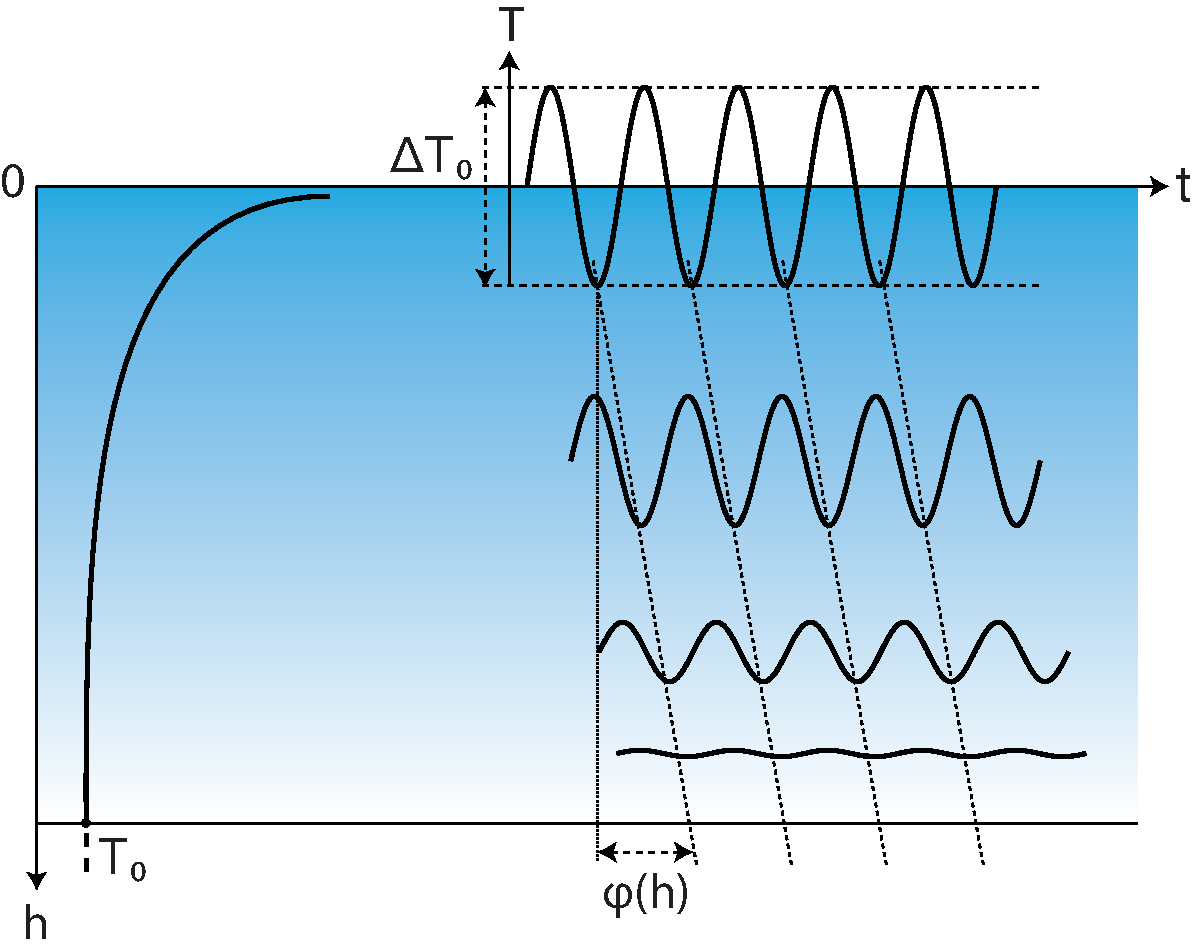
\includegraphics[width=8.25cm]{figures/temp-attenuation}
   \end{figure}
 \end{columns}  
\end{frame}


\begin{frame}
  \frametitle{Ice temperatures close to the glacier surface}
  \begin{columns}
    \column[T]{1.75cm} 
    \vspace{1cm}
    {\includegraphics<1>[width=1.5cm]{figures/glaciersv_c}}%
    \vspace{2.5cm}
    \column[T]{10.25cm}
    \begin{block}{Analytical Solution}
      \begin{equation*}
        \label{eq:heat-flow-1d-solution}
        T(h,t) = T_0 + \underbrace{\Delta T_0 \exp\left(-h \sqrt{\frac{\omega}{2\kappa}}\right)}_{\Delta T(h)}
        \sin\Big(\omega t - \underbrace{h \sqrt{\frac{\omega}{2\kappa}}}_{\varphi(h)}\Big).
      \end{equation*}
      \begin{tabular}{cl}
        $\Delta T(h)$ & amplitude variation with depth 
      \end{tabular}
    \end{block}
  \end{columns}  
\end{frame}


% \begin{frame}
%   \frametitle{Ice temperatures close to the glacier surface}
%   \begin{columns}
%     \column[T]{1.75cm} 
%     \vspace{1cm}
%     {\includegraphics<1>[width=1.5cm]{figures/glaciersv_c}}%
%     \vspace{2.5cm}
%     \column[T]{10.25cm}
%     \vspace{-1em}
%     \begin{figure}
%       \movie[width=7.cm,showcontrols=true]{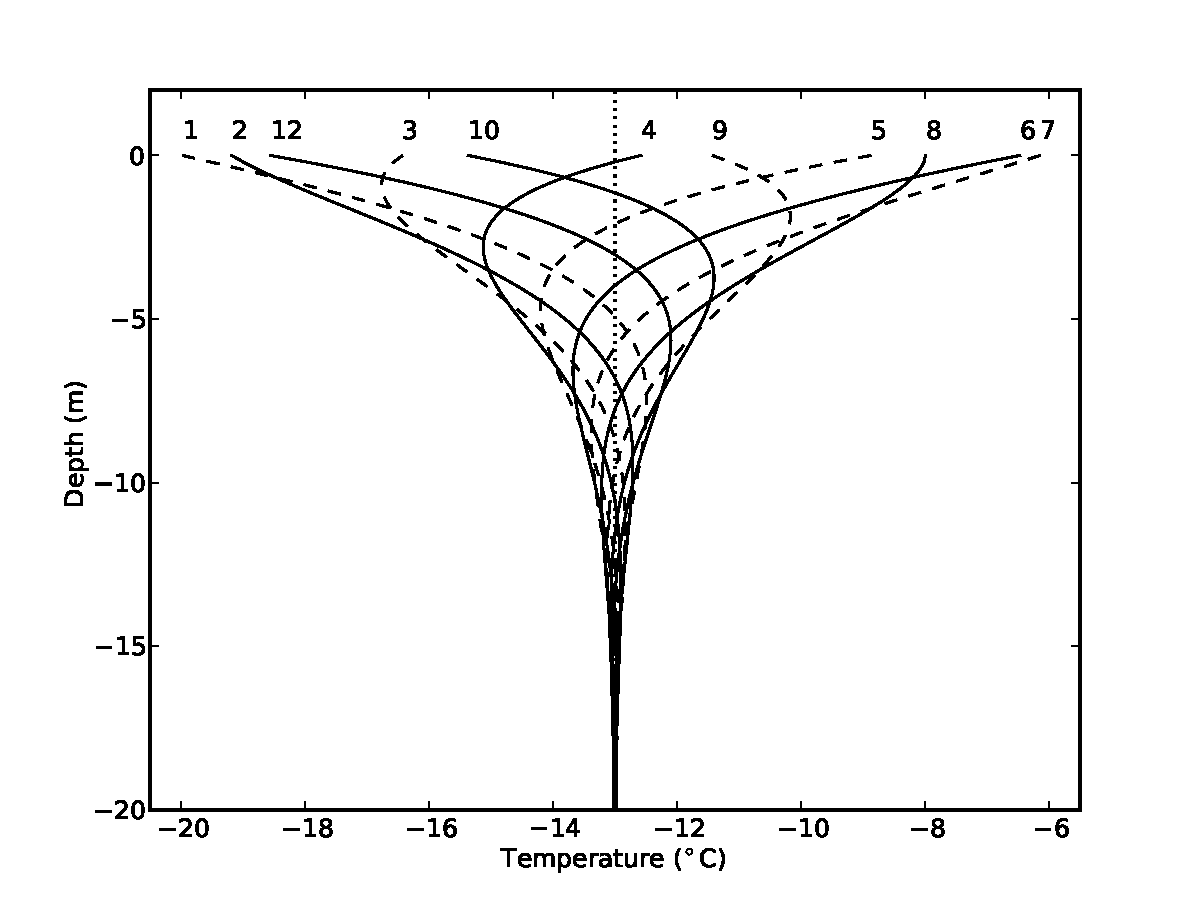
\includegraphics[width=7.cm]{figures/temp-variation}}{heat-flow-sinus-forcing.avi}
%       \caption{Simulated variation of temperature with depth for the conditions at Colle
%         Gnifetti. Numbers next to curves indicate months (1 corresponds to January).}
%     \end{figure}
%  \end{columns}  
% \end{frame}


\begin{frame}
  \frametitle{Ice temperatures close to ice divides}
  \begin{columns}
    \column[T]{1.75cm} 
    \vspace{1cm}
    {\includegraphics<1>[width=1.5cm]{figures/glaciersv_c}}%
    \vspace{2.5cm}
    \column[T]{10.25cm}
      % \begin{equation*}
      %   \label{eq:cold_pde}
      %   \rho c(T)\left(\ddt{T} + {\bf v}\cdot\nabla T\right) =  - \nabla \cdot {\bf q} + Q
      % \end{equation*}
      \begin{block}{Assumptions}
        \begin{itemize}
        \item only vertical advection and diffusion
       \end{itemize}
        We then get
    \begin{equation*}
      \label{eq:heat-diffusion-advection-1d-steady}
      \kappa \frac{\partial^2T}{\partial z^2} =  w(z) \ddz{T}
    \end{equation*}
        where $w$ is the vertical velocity
      \end{block}
      \begin{block}{Analytical solution}
        \begin{itemize}
        \item can be obtained
       \end{itemize}
     \end{block}
 \end{columns}  
\end{frame}


\subsubsection{Cold Glaciers}
\label{sec:cold-glaciers}

\begin{frame}
  \frametitle{Cold Glaciers}
  \begin{figure}
    \includegraphics<1>[height=4cm]{figures/taylor_valley}\vspace{.5em}
    \includegraphics<1>[height=4cm]{figures/Mcmurdo_sound_USGS_map}
  \end{figure}
  \begin{itemize}
  \item Dry Valleys, Antarctica
  \item (very) high altitudes at lower latitudes
  \end{itemize}
\end{frame}


\section{Temperate Ice}
\label{sec:temperate-ice}

\subsection{Equation}
\label{sec:temperate-ice-equation}

\begin{frame}
  \frametitle{Water content equation}
  \begin{columns}
    \column[T]{1.75cm}
    \vspace{1cm}
    {\includegraphics<1>[width=1.5cm]{figures/glaciersv_t}}%
    \vspace{2.5cm}
    \column[T]{10.25cm}
    \begin{block}{Water content equation}
      \begin{itemize}
      \item Ice is temperate if a change in heat content leads to a change in water content alone
      \item  independent variable: water content (aka moisture content, liquid water fraction) $\omega = L^{-1} u$
      \end{itemize}
      \begin{equation*}
        \label{eq:temperate_pde}
        \rho L\left(\frac{\partial \omega}{\partial t} + {\bf v}\cdot\nabla \omega\right)  = -\nabla \cdot {\bf q} + Q
      \end{equation*}
      $\Rightarrow$ in temperate ice, \alert{water content} plays the role of \alert{temperature}
    \end{block}
 \end{columns}
\end{frame}


\subsection{Flow law}
\label{sec:temperate-ice-flow-law}

\begin{frame}
  \frametitle{Flow law}
  \begin{columns}
    \column[T]{1.75cm} 
    \vspace{1cm}
    {\includegraphics<1>[width=1.5cm]{figures/glaciersv_t}}%
    \vspace{3cm}
    \column[T]{10.25cm}
    \begin{block}{Flow Law}
      Viscosity $\eta$ is a function of effective strain rate $d_{\text e}$ and water content $\omega$
      \begin{equation*}
        \eta = \eta(\omega,d_{\text e}) =1/2 B(\omega) d_{\text e}^{(1-n)/n}
     \end{equation*}
     where B depends \alert{linearly} on $\omega$
     \begin{itemize}
     \item but only very few studies (e.g. from Lliboutry and Duval)
     \end{itemize}
    \end{block}
  \begin{block}{Latent heat flux}
      \begin{equation*}
        \label{eq:enthalpy-flux-temperate}
        {\bf q}  = {\bf q}_{l} =
        \left\{
          \begin{array}{l}
            \textsf{Fick-type}  \\
            \textsf{Darcy-type} 
          \end{array}
        \right.
      \end{equation*}
      $\Rightarrow$ leads to different mixture theories (\emph{Class I}, \emph{Class II}, \emph{Class III}) 
   \end{block}
 \end{columns}
\end{frame}


\begin{frame}
  \frametitle{Sources for liquid water in temperate Ice}
  \vspace{-1em}
  \begin{figure}
    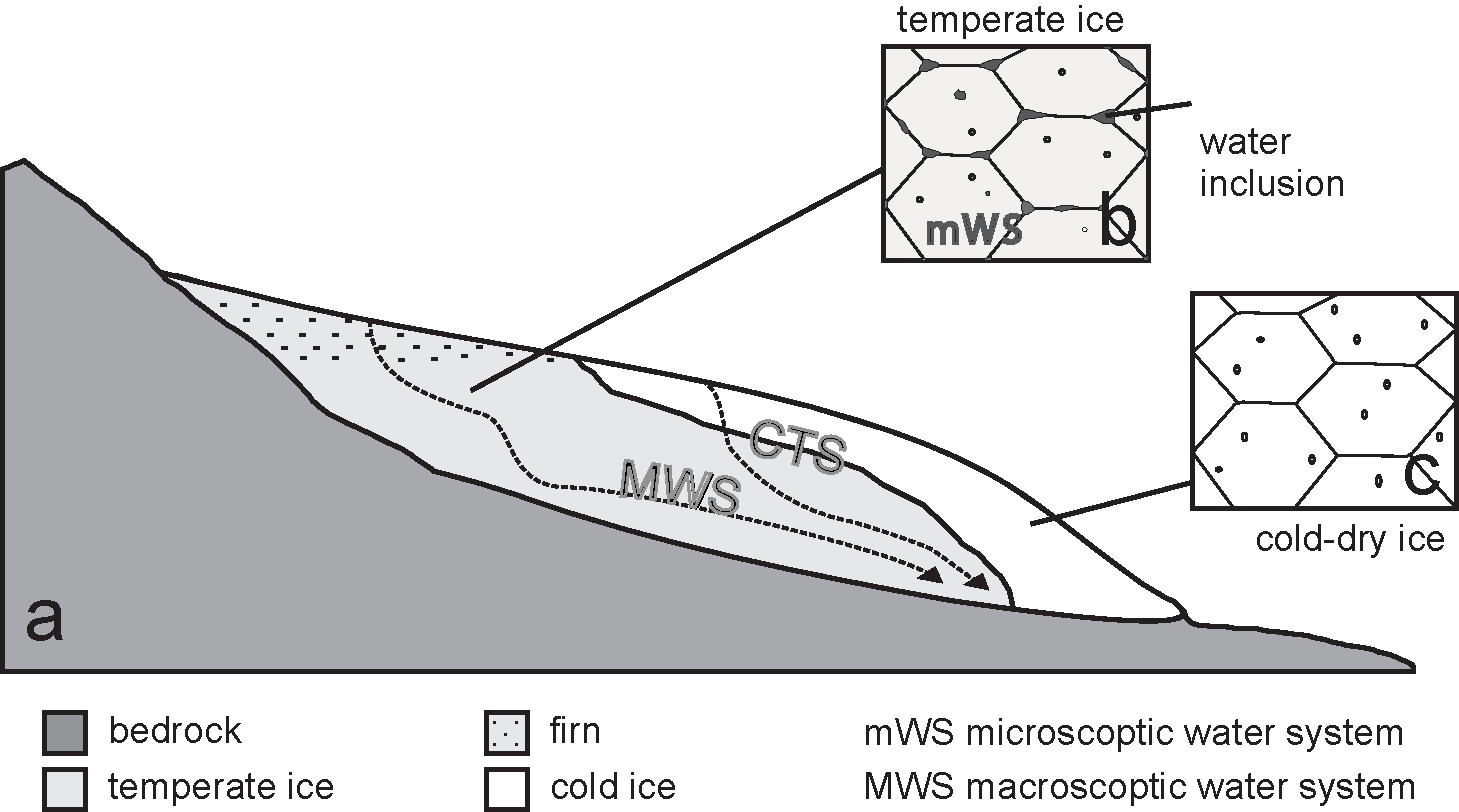
\includegraphics[width=8cm]{figures/mws}
  \end{figure}
  \begin{enumerate} \small
  \item<1-2> water trapped in the ice as water-filled pores
  \item<1-2> water entering the glacier through cracks and crevasses at the ice surface in the ablation area
  \item<1,3> changes in the pressure melting point due to changes in lithostatic pressure
  \item<1,3> melting due energy dissipation by internal friction (strain heating) 
  \end{enumerate}  
\end{frame}




\begin{frame}
  \frametitle{Temperature and water content of temperate ice}
  \begin{block}{Temperature}
    \begin{equation}
      \label{eq:clausius-pure}
      T_m = T_{\text{tp}} - \gamma\, (p - p_{\text{tp}})\,,
    \end{equation}
    \begin{itemize}
    \item $T_{\text{tp}}=273.16\unit{K}$ triple point temperature of water
    \item $p_{\text{tp}}=611.73\unit{Pa}$ triple point pressure of water
    \item Temperature follows the pressure field
    \end{itemize}
  \end{block}
  \begin{block}{Water content}
    \begin{itemize}
    \item generally between 0 and $3\%$
    \item water contents up to $9\%$ found
    \end{itemize}
  \end{block}
\end{frame}


\subsubsection{Temperate Glaciers}

\begin{frame}
  \frametitle{Temperate Glaciers}
  \begin{figure}
    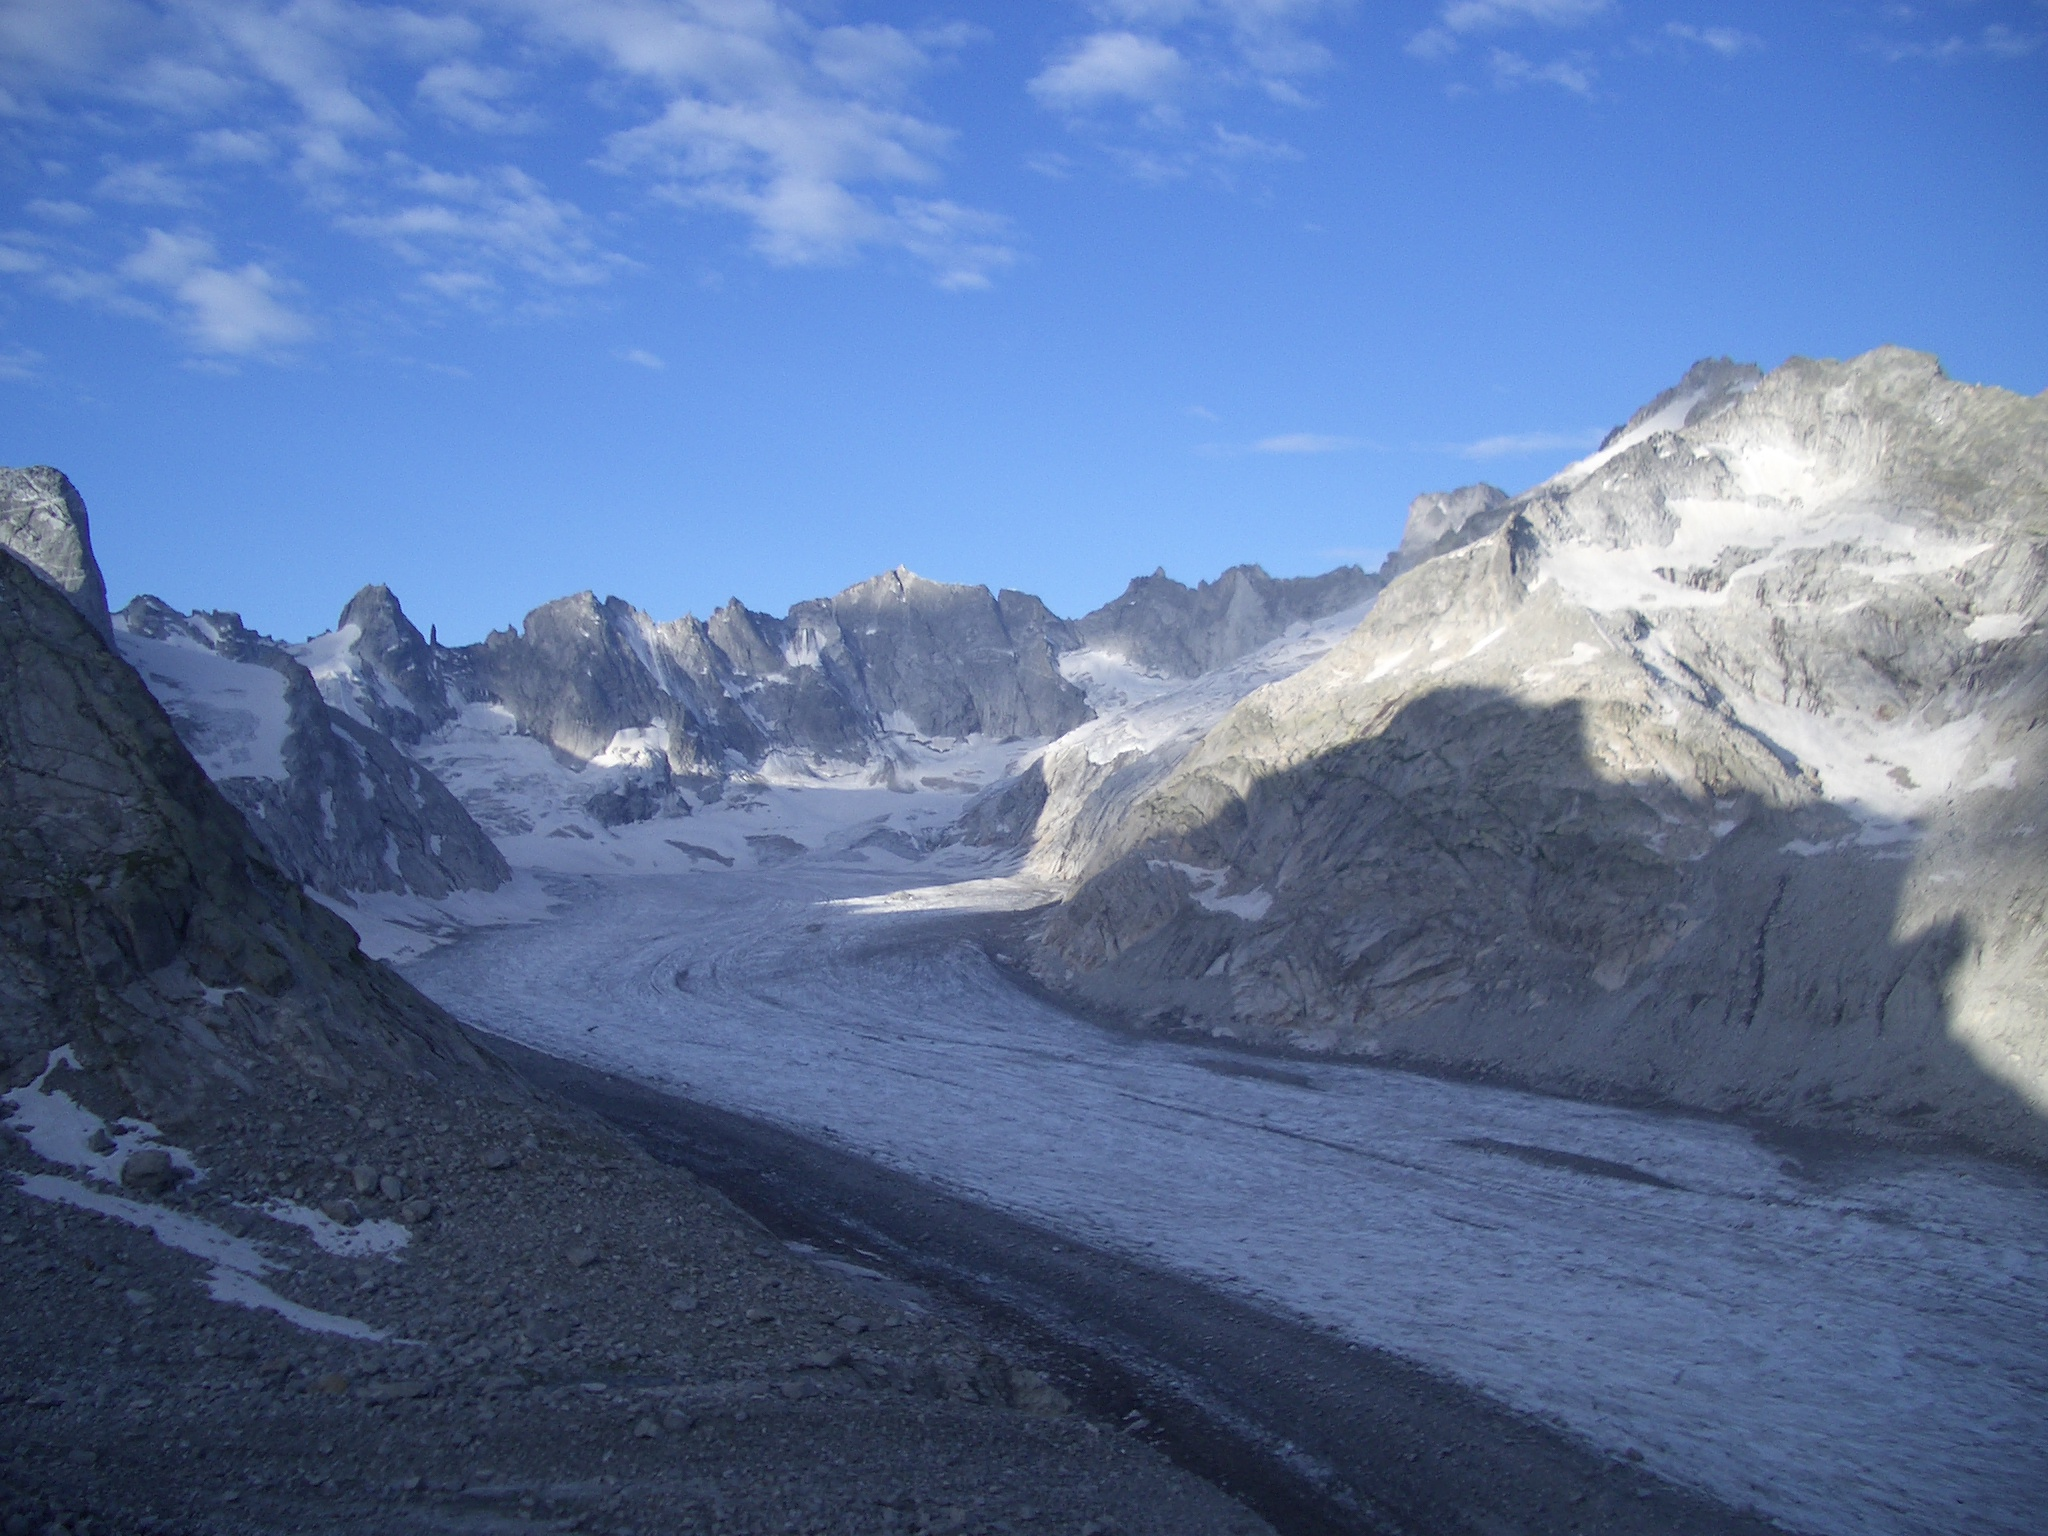
\includegraphics[width=5cm]{figures/forno}
  \end{figure}
  Temperate glaciers are widespread, e.g.:
  \begin{itemize}
  \item Alps, Andes, Alaska,
  \item Rocky Mountains, tropical glaciers, Himalaya
  \end{itemize}
\end{frame}


\section{Polythermal Glaciers}


% \begin{frame}
%   \frametitle{Polythermal Glaciers}
%   \begin{columns}
%     \column[T]{1.75cm} 
%     \vspace{1cm}
%     {\includegraphics<1>[width=1.5cm]{figures/glaciersv_p}}%
%     \vspace{2.5cm}
%     \column[T]{10.25cm}
%   \begin{figure}
%     {\includegraphics<1>[width=9cm]{figures/mws}}%
%     \caption{Gusermeroli et al. (2010), modified}
%   \end{figure}
%   \note{
% mWS consists of ($\mu$m-scale) water inclusions found in veins and nodes along three grain intersections, lenses on grain boundaries and in irregular shapes [Raymond and Harrison, 1975; Nye, 1989; Mader, 1992; Fountain and Walder, 1998]. Such water inclusions are primarily generated in the accumulation area, where meltwater percolates through the porous firn and becomes part of the glacier-ice crystalline structure when the pores close by compaction [Paterson, 1971;Lliboutry, 1976; Pettersson et al., 2004].
% }
%   \end{columns}
% \end{frame}


\begin{frame}
  \frametitle{Polythermal glaciers}
  \begin{columns}
    \column[T]{1.75cm} 
    \vspace{1cm}
    {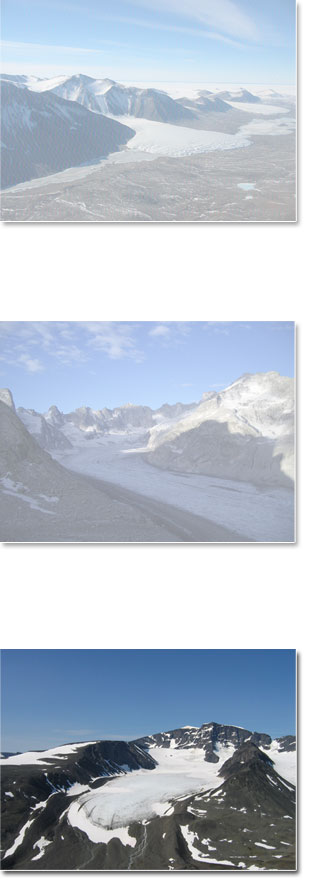
\includegraphics[width=1.5cm]{figures/glaciersv_p}}%
    \vspace{2.5cm}
    \column[T]{10.25cm}
  \begin{figure}
    \includegraphics<1>[width=10cm]{figures/CTSstructures-2land}
 \end{figure}
    \begin{itemize}
    \item contains both cold and temperate ice
    \item separated by the cold-temperate transition surface (CTS)
    \item CTS is an internal free surface of discontinuity where phase changes may occur
    \item polythermal glaciers, but \alert{not} polythermal ice
    \end{itemize}
  \end{columns}
\end{frame}


\subsection{Thermal Structures}

\begin{frame}
  \frametitle{Scandinavian-type thermal structure}
  \begin{columns}
    \column[T]{1.75cm} 
    \vspace{1cm}
    {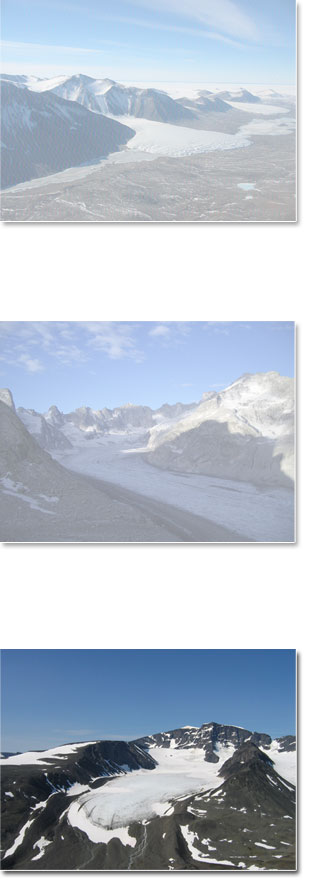
\includegraphics[width=1.5cm]{figures/glaciersv_p}}%
    \vspace{2.5cm}
    \column[T]{10.25cm}
  \begin{figure}
    \includegraphics<1>[width=10cm]{figures/CTSstructures-2land}
 \end{figure}
  \begin{itemize}
  \item Scandinavia
  \item Svalbard
  \item Rocky Mountains
  \item Alaska
  \item Antarctic Peninsula
  \end{itemize}
  \end{columns}
\end{frame}


\begin{frame}
  \frametitle{Scandinavian-type thermal structure}
  \begin{columns}
    \column[T]{1.75cm} 
    \vspace{1cm}
    {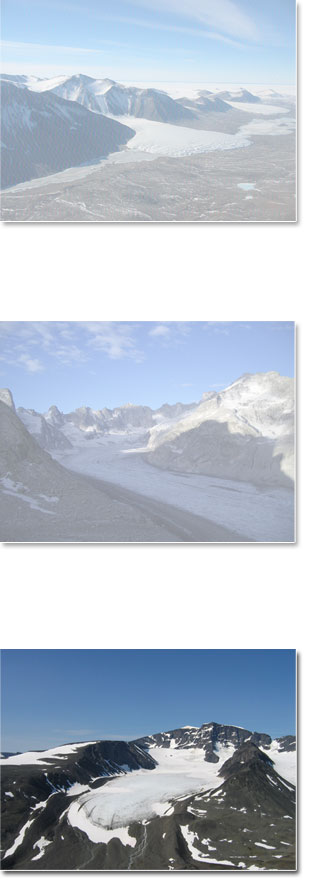
\includegraphics[width=1.5cm]{figures/glaciersv_p}}%
    \vspace{2.5cm}
    \column[T]{10.25cm}
    Why is the surface layer in the ablation area cold? Isn't this counter-intuitive?
    \begin{figure}
      \includegraphics<1>[width=9.5cm]{figures/CTS_scandic}
    \end{figure}
  \end{columns}
\end{frame}


\begin{frame}
 \frametitle{Canadian-type thermal structure}
  \begin{columns}
    \column[T]{1.75cm} 
    \vspace{1cm}
    {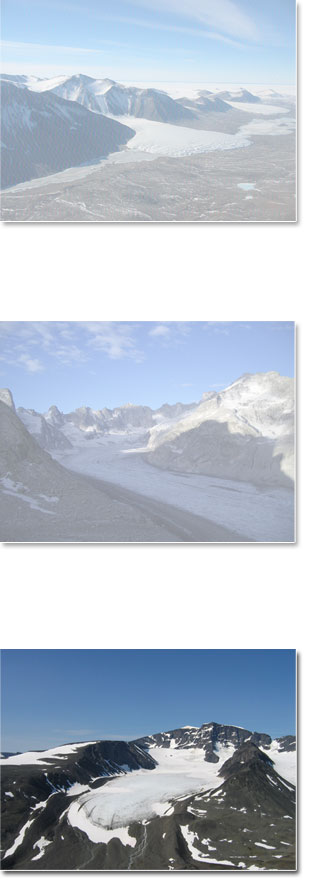
\includegraphics[width=1.5cm]{figures/glaciersv_p}}%
    \vspace{2.5cm}
    \column[T]{10.25cm}
    \begin{figure}
      \includegraphics<1>[width=10cm]{figures/CTSstructures-2land}
    \end{figure}
    \begin{itemize}
    \item high Arctic latitudes in Canada
    \item Alaska
    \item both ice sheets Greenland and Antartica
    \end{itemize}
  \end{columns}
\end{frame}



\section{Ice Sheet Models}


\begin{frame}
  \frametitle{Thermodynamics in ice sheet models}
  \begin{itemize}
  \item only few glaciers are completely cold
  \item most ice sheet models are so-called \emph{cold-ice method} models
  \item so far two polythermal ice sheet models
  \end{itemize}
      \begin{align*}
       \rho c(T)\left(\ddt{T} + {\bf v}\cdot\nabla T\right) & =  \nabla \cdot k \nabla T + Q \\
       \rho\,L\left(\ddt{\omega} + {\bf v}\cdot\nabla \omega \right) & =   Q
      \end{align*}
      or
     \begin{align*}
       \rho \left(\ddt{E} + {\bf v}\cdot\nabla E\right) & =  \nabla \cdot \nu \nabla E + Q
     \end{align*}
\end{frame}

\begin{frame}
  \frametitle{Thermodynamics in ice sheet models}
  \begin{block}{Cold vs Polythermal for Greenland}
  \begin{itemize}
  \item better conservation of energy
    \item more realistic basal melt rates
      well-defined interfaces to the atmosphere and subglacial hydrology
    \end{itemize}
   \end{block}	
\end{frame}


\begin{frame}{Why polythermal is better: Antarctica}
\begin{columns}[c]
    \begin{column}{.3\linewidth}
      \begin{itemize}
      \item conservation of energy
      \item more realistic basal melt rates
      \item more realistic ice streams
      \end{itemize}
    \end{column}
    \begin{column}{.7\linewidth}
      \vspace{-.5cm}
      \begin{figure}
        \only<1>{\small{\alert{temperature equation}} \\}
        \only<2>{\small{\alert{enthalpy equation}} \\}
        {\footnotesize basal melt rate, meters per year}\\
        \includegraphics<1>[width=.9\textwidth]{figures/ant_bmelt_temp}
        \includegraphics<2>[width=.9\textwidth]{figures/ant_bmelt_enth} \\
        {\small M. Martin, PIK}
      \end{figure}
    \end{column}
  \end{columns}
\end{frame}


\begin{frame}{Why polythermal is better: Greenland}
\begin{columns}[c]
    \begin{column}{.3\linewidth}
      \begin{itemize}
      \item conservation of energy
      \item more realistic basal melt rates
      \item more realistic ice streams
      \end{itemize}
    \end{column}
    \begin{column}{.7\linewidth}
      \vspace{-.5cm}
      \begin{figure}
        \only<1>{\small{\alert{temperature equation}} \\}
        \only<2>{\small{\alert{enthalpy equation}} \\}
        {\footnotesize basal melt rate, meters per year}\\
        \includegraphics<1>[width=.5\textwidth]{figures/grn_bmelt_temp}
        \includegraphics<2>[width=.5\textwidth]{figures/grn_bmelt_enth} \\
     \end{figure}
    \end{column}
  \end{columns}
\end{frame}

\end{document}
